% Provenance (never printed): see sources/outline_sources.md (Year 1: morphology,
% gravity, heat flow and seismicity of a subduction zone; accretionary and erosive
% margins; slab geometry; volcanic arcs). Kuril map, section and numbers from
% figdata/bachelor-1/slab_seismicity.py; exercise and problem values in the Book 3
% scratch calculator calc/ch14.py.
\chapter{Actieve randen}\label{ch:b1:active-margins}

Op 11 maart 2011, om 14.46 uur plaatselijke tijd, brak de plaatgrens voor het noordoosten van Japan over ongeveer \qty{400}{km} langs de trog en \qty{150}{km} naar beneden langs haar helling. De breuk gleed tot wel 50 tot \qty{60}{m}, meest omhoog langs de helling van het hypocentrum, richting de Japantrog; op het land bewoog de kust horizontaal en zakte zij. De plaat die daar zinkt, de Pacifische plaat, gaat onder Japan naar beneden langs een vlak dat aardbevingen tot honderden kilometers diep omlijnen; en waar dat vlak ongeveer honderd kilometer diep ligt, loopt een reeks vulkanen evenwijdig aan de kust. Dit hoofdstuk leest zo'n rand af aan haar vorm, haar zwaartekracht, haar \omterm{def:b1:heat-budget:heat-flow}{warmtestroom} en, bovenal, haar aardbevingen.
% ledger: usgs:tohoku, wada:decoupling

\begin{recall}
Oceanische litosfeer zinkt bij subductiezones terug in de \omterm{def:b1:layered-earth:layers}{mantel}, gemarkeerd door trogs en door schuine zones van aardbevingen, en oude litosfeer zinkt onder haar eigen gewicht (Boek 2, klas 11); water uit de zinkende plaat verlaagt de smelttemperatuur van de \omterm{def:b1:layered-earth:layers}{mantel} erboven (Boek 2, klas 12). Warmte diffundeert over een afstand $L$ in een tijd van de orde $L^2/\kappa$ (\cref{ch:b1:heat-budget}); een oneindige plaat van dichtheid $\rho$ en dikte $h$ trekt aan met $2\pi G\rho h$ (\cref{ch:b1:isostasy-gravity}); platen bewegen om Eulerpolen (\cref{ch:b1:plate-kinematics}); de \omterm{def:b1:heat-budget:heat-flow}{warmtestroom} van de oceaanbodem daalt als de inverse vierkantswortel van haar leeftijd (\cref{ch:b1:rifts-ridges-margins}).
\end{recall}

\section{De anatomie van een actieve rand}\label{sec:b1:active-margins:anatomy}

\begin{definition}[Actieve rand, oceanische trog, voorboog, achterboogbekken]\label{def:b1:active-margins:active-margin}
Een \emph{actieve rand}\index{actieve rand} is een convergente plaatgrens waar oceanische litosfeer onder een andere plaat wegzakt, hetzij onder een continent, hetzij onder een andere oceanische plaat. Een \emph{oceanische trog}\index{oceanische trog} is de lange, smalle, V-vormige inzinking van de zeebodem waarlangs de zinkende plaat omlaag buigt onder de andere. De \emph{voorboog}\index{voorboog} is het deel van de bovenliggende plaat tussen de trog en de rij vulkanen. Een \emph{achterboogbekken}\index{achterboogbekken} is een bekken achter de vulkanen, aan de kant weg van de trog, waar de bovenliggende plaat wordt uitgerekt en nieuwe \omterm{def:b1:rifts-ridges-margins:oceanic-crust}{oceanische korst} zich kan vormen.
\end{definition}

Troggen zijn de diepste plaatsen van de oceanen, en de diepste van alle is de Challenger Deep van de Marianentrog. Over de Koeriletrog daalt de bodem van ongeveer \qty{5200}{m} op de abyssale vlakte tot \qty{8700}{m} in de as, ongeveer \qty{3.5}{km} lager, en is de trog slechts tientallen kilometers breed (figuur in \cref{sec:b1:active-margins:gravity-heat}). De convergente randen van de aarde meten samen ongeveer \qty{55000}{km}; in een digitaal model van de plaatgrenzen tellen de subductiegrenzen op tot ongeveer \qty{51000}{km}, tegenover ongeveer \qty{67000}{km} aan spreidingsruggen.
% ledger: data:b3-grav-kuril (trench_gravity.py values), stern:subduction, data:pb2002 (ridge_budget.py)

Voor de trog buigt de plaat iets omhoog voordat zij duikt, in een brede, lage buitenrug. Daar is de plaat gebogen, en is haar bovenste deel uitgerekt: aardbevingen met normale breukbeweging treffen de buitenruggen. De breedte van de buitenrug komt overeen met de buiging van een elastische plaat; deze buiging van de litosfeer wordt bestudeerd in Boek 5. De trog zelf is de plaats waar het gewicht van de dichte zinkende plaat de voorrand naar beneden trekt.

\begin{definition}[Subducerende plaatzijde]\label{def:b1:active-margins:slab}
De \emph{subducerende plaatzijde}\index{subducerende plaatzijde} is het deel van de zinkende plaat dat al de \omterm{def:b1:layered-earth:layers}{mantel} in is gegaan: een vel oceanische litosfeer, met haar \omterm{def:b1:layered-earth:layers}{korst} erop, schuin onder de bovenliggende plaat van de trog tot diepten van enkele honderden kilometers.
\end{definition}

De bovenliggende plaat is in stroken evenwijdig aan de trog gesneden (figuur hieronder): de \omterm{def:b1:active-margins:active-margin}{voorboog}, vaak met een stapel afgeschraapte sedimenten aan haar voorkant en een sedimentbekken erachter; de \omterm{def:b1:active-margins:volcanic-arc}{vulkanische boog}; en, achter sommige bogen, een \omterm{def:b1:active-margins:active-margin}{achterboogbekken} en een oudere, uitgedoofde boog daarachter. Tussen de plaatzijde en de bovenliggende plaat ligt een wig van \omterm{def:b1:layered-earth:layers}{mantel}, meegesleept langs de bovenkant van de plaatzijde.

\begin{omfigure}
\begin{tikzpicture}[x=0.01667cm, y=0.01667cm, font=\scriptsize,
  lbl/.style={fill=white, fill opacity=0.8, text opacity=1, inner sep=1pt}]
\begin{scope}
\clip (-150,-330) rectangle (650,55);
% mantle and sea water
\fill[orange!12] (-150,-330) rectangle (650,15);
\fill[omSea!45] (-150,15) rectangle (650,0);
% incoming plate and slab: top dips 25 deg to 50 km, then 45 deg; 100 km thick
\fill[omLithBasalt!55] (-150,4) -- (-80,4) .. controls (-60,7) and (-40,7) .. (-25,4) -- (0,0)
  -- (107.2,-50) -- (420,-363) -- (349,-434) -- (48.9,-133.1) -- (-22.1,-100) -- (-150,-100) -- cycle;
\draw[omSea!50!black, line width=1.6pt] (-150,4) -- (-80,4) .. controls (-60,7) and (-40,7) .. (-25,4) -- (0,0) -- (107.2,-50) -- (420,-363);
% overriding plate
\fill[brown!28] (0,0) -- (12,3) -- (45,8) -- (60,10) -- (140,10) -- (150,12) -- (184,12) -- (230,9)
  -- (300,7) -- (395,6) -- (410,3) -- (420,2) -- (430,3) -- (445,6) -- (540,7) -- (560,14) -- (590,14)
  -- (610,10) -- (650,10) -- (650,-60) -- (520,-55) -- (445,-25) -- (420,-15) -- (395,-25) -- (320,-55)
  -- (250,-60) -- (117.2,-60) -- (107.2,-50) -- cycle;
% accretionary prism and forearc basin
\fill[yellow!55] (0,0) -- (12,3) -- (45,8) -- (60,10) -- (60,-28) -- cycle;
\draw[black!45, line width=0.3pt] (14,-3) -- (24,5) (28,-7) -- (38,6) (42,-14) -- (52,8);
\fill[yellow!30] (68,10) -- (132,10) -- (122,4) -- (78,4) -- cycle;
% arc volcano
\fill[black!60] (150,12) -- (167,26) -- (184,12) -- cycle;
% an isotherm: a cold tongue down the slab
\draw[omDef, dashed, line width=0.6pt] (-150,-82) -- (-30,-82) -- (40,-118) -- (300,-318)
  -- (232,-200) -- (150,-112) .. controls (130,-80) and (180,-72) .. (260,-72) -- (650,-72);
% mantle wedge flow
\draw[->, black!60, line width=0.5pt] (600,-130) .. controls (450,-135) and (300,-125) .. (215,-150)
  .. controls (205,-160) and (240,-185) .. (300,-235);
% water and melt
\foreach \x/\z in {150/-93, 172/-115, 194/-137}
  \draw[->, blue!70!black, line width=0.5pt] (\x,\z) -- (\x-6,\z+28);
\draw[red!75!black, line width=0.8pt, decorate, decoration={snake, amplitude=1.2, segment length=6}] (167,-100) -- (167,12);
% earthquakes
\foreach \x/\z in {20/-12, 45/-22, 70/-34, 95/-45, 60/-40, 85/-58, 120/-70, 135/-85, 150/-104,
  165/-112, 185/-140, 205/-150, 225/-175, 248/-195, 270/-216, 290/-242, 312/-262, 330/-282, 350/-300, 365/-318}
  \fill[black] (\x,\z) circle[radius=0.9pt];
% the 100-km level beneath the arc
\draw[black!70, densely dotted] (90,-100) -- (260,-100);
\draw[black!70, densely dotted] (167,12) -- (167,-110);
\end{scope}
\draw[black!70] (-150,-330) rectangle (650,55);
\node[lbl, anchor=south] at (-85,15) {buitenrug};
\node[lbl, anchor=south] at (0,15) {trog};
\node[lbl, anchor=west] (pr) at (75,-28) {accretionair prisma};
\draw[black!70] (pr.west) -- (38,-6);
\node[lbl, anchor=south] at (88,15) {voorboog};
\node[lbl, anchor=south] at (185,27) {vulkanische boog};
\node[lbl, anchor=south] at (420,15) {achterboogbekken};
\node[lbl, anchor=south] at (575,15) {overblijfsel van de boog};
\node[lbl, anchor=west] at (-140,-50) {oceanische litosfeer};
\node[lbl, anchor=east] (sl) at (120,-262) {subducerende plaatzijde};
\draw[black!70] (sl.east) -- (205,-262);
\node[lbl, anchor=west] (wb) at (420,-265) {Wadati--Benioff-zone};
\draw[black!70] (wb.west) -- (318,-266);
\node[lbl] at (430,-170) {mantelwig};
\node[lbl] at (575,-30) {bovenliggende plaat};
\node[lbl, anchor=west, text=blue!70!black] at (212,-98) {water};
\node[lbl, anchor=east] at (88,-100) {\qty{100}{km} diep};
\node[lbl, anchor=west, text=omDef] at (450,-95) {een isotherm};
\node[lbl, anchor=west] at (-140,-300) {mantel};
\draw[line width=1pt] (500,-310) -- (600,-310) node[midway, above] {\qty{100}{km}};
\end{tikzpicture}
\par\smallskip{\small Een subductiezone in doorsnede (schematisch: litosfeer en plaatzijde getekend op de schaalbalk, reliëf boven de zeebodem sterk overdreven). De plaatzijde helt flauw onder de \omterm{def:b1:active-margins:active-margin}{voorboog} en steiler eronder; de \omterm{def:b1:active-margins:volcanic-arc}{vulkanische boog} staat boven de plaats waar de bovenkant van de plaatzijde ongeveer \qty{100}{km} diep ligt. De koude plaatzijde sleept haar isothermen de \omterm{def:b1:layered-earth:layers}{mantel} in (gestippeld: één isotherm), en de \omterm{def:b1:layered-earth:layers}{mantel} van de wig wordt langs haar naar beneden meegesleept. Stippen: aardbevingen, op de plaatgrens nabij de trog en in de plaatzijde eronder. Water dat door de plaatzijde vrijkomt, stijgt op in de wig; smelt stijgt op naar de boog.}
\label{fig:b1:active-margins:section}
\end{omfigure}

Opgeteld over hetzelfde digitale model gaan elk jaar ongeveer \qty{2.7}{km^2} oceaanbodem naar de subductiegrenzen, dicht bij de \qty{3.0}{km^2} die bij de ruggen worden gemaakt (\cref{ch:b1:rifts-ridges-margins}): binnen de nauwkeurigheid van zo'n model, dat de trage vervorming van brede plaatgrenszones buiten beschouwing laat, wordt de oceaanbodem even snel vernield als zij wordt gemaakt, en behoudt het aardoppervlak zijn grootte.
% ledger: data:pb2002 (ridge_budget.py: consumed 2.74, made 3.01 km2/yr)

\section{Zwaartekracht en warmtestroom}\label{sec:b1:active-margins:gravity-heat}

Felix Vening Meinesz vond de lange, smalle gordels van negatieve zwaartekrachtsanomalieën langs de trogs (\cref{ch:b1:isostasy-gravity}). Satellieten brengen ze nu overal op zee in kaart. Over de Koeriletrog (figuur hieronder) stijgt de \omterm{def:b1:isostasy-gravity:anomalies}{vrije-luchtanomalie} tot ongeveer \qty{40}{\milli\gal} boven de buitenrug, daalt zij tot \qty{-260}{\milli\gal} boven de trog, en is zij in de \omterm{def:b1:active-margins:active-margin}{voorboog} en de eilanden van de boog weer sterk positief.
% ledger: egs:vening-meinesz, data:b3-grav-kuril (trench_gravity.py values: rise 38 mGal at -155 km, low -260 at 0, high 218 at 160 km)

De grootte van de anomalie boven de trog zegt hoe de trog wordt gedragen. Stel dat de trog, \qty{3.5}{km} dieper dan de bodem eromheen, helemaal niet gecompenseerd was: waar de trog ligt, wordt \qty{3.5}{km} gesteente van dichtheid ongeveer \qty{2700}{kg.m^{-3}} vervangen door zeewater. Volgens de Bouguer-plaat (\cref{prop:b1:isostasy-gravity:slab}) zou de zwaartekracht daar lager zijn met
\[
  2\pi G\,\Delta\rho\,h = 2\pi \times \num{6.674e-11} \times 1700 \times 3500
  \approx \qty{2.5e-3}{m.s^{-2}} = \qty{250}{\milli\gal} .
\]
Dat is de grootte van de waargenomen laagte. Een trog is dus niet in isostatisch evenwicht: zij is een inzinking die omlaag wordt gehouden, door de sterkte van de gebogen plaat en door de trek van de plaatzijde, tegen het opwaartse vermogen van de \omterm{def:b1:layered-earth:layers}{mantel} eronder. (Een trog die slechts tientallen kilometers breed is, trekt minder aan dan een oneindige plaat, dus het water erin alleen geeft iets minder dan dit; het overige tekort ligt dieper, waar de hele gebogen plaat, met haar lichte \omterm{def:b1:layered-earth:layers}{korst} erbij, de \omterm{def:b1:layered-earth:layers}{mantel} in wordt gedrukt: oefening~\ref{exo:b1:active-margins:1}.)

\begin{omfigure}
\begin{tikzpicture}
\begin{axis}[omrecord, name=grav, width=0.86\linewidth, height=4.6cm, xmin=-250, xmax=450,
  ymin=-300, ymax=260, ylabel={vrije lucht (\unit{\milli\gal})}, ylabel style={at={(-0.075,0.5)}}, xticklabels={},
  ytick={-200,-100,0,100,200}, clip=false]
% computed in figdata/bachelor-1/trench_gravity.py; ledger: data:b3-grav-kuril
\addplot[black!30, forget plot] coordinates {(-250,0) (450,0)};
\addplot[omDef, line width=1pt] table[x=x, y=faa] {figdata/out/bachelor-1-trench_gravity-profile.dat};
\draw[black!50, densely dotted] (axis cs:0,-300) -- (axis cs:0,260) (axis cs:164,-300) -- (axis cs:164,260);
\node[font=\scriptsize, anchor=south] at (axis cs:-155,45) {buitenrug, $+38$};
\node[font=\scriptsize, anchor=west] at (axis cs:12,-262) {trog, $-260$};
\node[font=\scriptsize, anchor=south west] at (axis cs:200,140) {voorboog en boog};
\end{axis}
\begin{axis}[omrecord, at={(grav.south)}, anchor=north, yshift=-0.45cm, width=0.86\linewidth, height=4.6cm,
  xmin=-250, xmax=450, ymin=20, ymax=100, ylabel={warmte (\unit{mW.m^{-2}})}, ylabel style={at={(-0.075,0.5)}},
  xlabel={afstand tot de trog, naar de bovenliggende plaat (\unit{km})}, clip=false]
% schematic; levels from the ledger: parsons:plate-model (11.3/sqrt(122) x 41.84 = 42.8 mW/m2 for the
% 122-Myr Kuril plate), hyndman:backarc (70-85); the forearc low is drawn without a value (wada:decoupling)
\addplot[fill=omDef!15, draw=none, forget plot] coordinates {(190,70) (450,70) (450,85) (190,85)} -- cycle;
\addplot[omProp!80!black, line width=1pt, smooth, tension=0.5] coordinates {(-250,43) (-60,43) (-10,41) (30,36) (120,36)
  (150,48) (180,76) (230,78) (450,78)};
\draw[black!50, densely dotted] (axis cs:0,20) -- (axis cs:0,100) (axis cs:164,20) -- (axis cs:164,100);
\node[font=\scriptsize, anchor=south] at (axis cs:-130,44) {oude oceaanbodem, ongeveer 43};
\node[font=\scriptsize, anchor=north] at (axis cs:75,34) {voorboog: lager};
\node[font=\scriptsize, anchor=south] at (axis cs:320,85) {boog en achterboogbekken, 70 tot 85};
\node[font=\scriptsize, anchor=north west] at (axis cs:3,99) {trog};
\node[font=\scriptsize, anchor=north west] at (axis cs:167,99) {boog};
\end{axis}
\end{tikzpicture}
\par\smallskip{\small Zwaartekracht en \omterm{def:b1:heat-budget:heat-flow}{warmtestroom} over een subductiezone. Boven: de vrije-luchtzwaartekrachtsanomalie, door satellieten gemeten over de Koeriletrog, langs de doorsnede van de figuur in \cref{sec:b1:active-margins:seismicity}: \qty{38}{\milli\gal} boven de buitenrug, \qty{-260}{\milli\gal} boven de trog, sterk positief boven de \omterm{def:b1:active-margins:active-margin}{voorboog} en de eilanden. Onder: de \omterm{def:b1:heat-budget:heat-flow}{warmtestroom}, een schematisch profiel: ongeveer \qty{43}{mW.m^{-2}} op de oude oceaanbodem, lager boven de \omterm{def:b1:active-margins:active-margin}{voorboog}, 70 tot \qty{85}{mW.m^{-2}} gemiddeld boven de boog en het \omterm{def:b1:active-margins:active-margin}{achterboogbekken}. Gestippeld: de trog en het vulkanische front. Gegevens: Scripps Institution of Oceanography marine zwaartekrachtmodel (Sandwell en anderen, 2014).}
\label{fig:b1:active-margins:profiles}
\end{omfigure}

De \omterm{def:b1:heat-budget:heat-flow}{warmtestroom} vertelt hetzelfde verhaal van de andere kant. De oude oceaanbodem die bij een trog aankomt, verliest weinig warmte: ongeveer \qty{43}{mW.m^{-2}} volgens de wet van \cref{ch:b1:rifts-ridges-margins} voor de Koerilese plaat, \qty{122}{Myr} oud. Boven de \omterm{def:b1:active-margins:active-margin}{voorboog} is de stroom nog lager: de koude plaatzijde eronder neemt warmte van boven op, en de \omterm{def:b1:layered-earth:layers}{mantel} onder de \omterm{def:b1:active-margins:active-margin}{voorboog} is koud en stilstaand. Boven de boog en het \omterm{def:b1:active-margins:active-margin}{achterboogbekken} is zij hoog, gemiddeld 70 tot \qty{85}{mW.m^{-2}}, tweemaal de stroom van de oude binnenlanden van continenten (ongeveer \qty{40}{mW.m^{-2}}). Een actieve \omterm{def:b1:active-margins:volcanic-arc}{vulkanische boog} heeft een mantelwig van ongeveer \qty{1200}{\celsius} nodig, op ongeveer \qty{100}{km} diepte; achter de boog is het hele \omterm{def:b1:active-margins:active-margin}{achterboogbekken} heet, met een litosfeer van slechts 50 tot \qty{60}{km} dik en een \omterm{def:b1:layered-earth:discontinuity}{Moho} op 800 tot \qty{900}{\celsius}.
% ledger: parsons:plate-model (11.3/sqrt(122) x 41.84 = 42.8), wada:decoupling, hyndman:backarc

Waarom blijft de plaatzijde koud? Zij zinkt sneller dan zij kan opwarmen. De Koerilese plaatzijde van \cref{sec:b1:active-margins:seismicity} komt de \omterm{def:b1:layered-earth:layers}{mantel} in met ongeveer \qty{82}{mm} per jaar en helt onder \ang{45}: zij bereikt \qty{600}{km} na een weg van $600/\sin\ang{45} \approx \qty{850}{km}$, in ongeveer tien miljoen jaar. Volgens de geleidingstijdschaal (\cref{prop:b1:heat-budget:timescale}) steekt warmte uit de \omterm{def:b1:layered-earth:layers}{mantel} de \qty{50}{km} over naar het midden van een plaatzijde van \qty{100}{km} dik in
\[
  \tau = \frac{L^2}{\kappa} = \frac{(\qty{5e4}{m})^2}{\qty{e-6}{m^2.s^{-1}}}
  = \qty{2.5e15}{s} \approx \qty{80}{Myr},
\]
ongeveer acht keer zo lang. De kern van de plaatzijde bereikt \qty{600}{km} bijna even koud als op de trog, en de isothermen worden met haar naar beneden meegesleept, zoals de doorsnede van een subductiezone hierboven laat zien.
% values (slab_seismicity.py): vel_normal 81.66 mm/yr, dip 44.9; calc/ch14.py

\section{Aardbevingen en de vorm van de plaatzijde}\label{sec:b1:active-margins:seismicity}

\begin{definition}[Wadati--Benioff-zone]\label{def:b1:active-margins:wadati-benioff}
Een \emph{Wadati--Benioff-zone}\index{Wadati--Benioff-zone} is de schuine zone van aardbevingen die nabij een trog begint en onder de bovenliggende plaat dieper wordt, tot wel ongeveer \qty{700}{km}: zij omlijnt de \omterm{def:b1:active-margins:slab}{subducerende plaatzijde}.
\end{definition}
% ledger: usgs:deepest

Haar aardbevingen zijn van twee soorten. Tot enkele tientallen kilometers diep komen zij voor op de plaatgrens zelf, de flauw hellende breuk waarlangs de twee platen langs elkaar schuiven; de grootste aardbevingen op aarde, zoals die van 2011 voor Japan, breken deze breuk. Dieper komen zij voor in de plaatzijde zelf, die alleen nog koud genoeg is om spanning op te slaan. Op de grootste diepten zou zelfs de plaatzijde eerder vloeien dan breken, en hoe diep aardbevingen beginnen, is nog omstreden. De diepste aardbeving van de catalogus, van magnitude 4.2, trof in 2004 onder de regio Vanuatu op \qty{735.8}{km}. In elke onderzochte subductiezone is de zone op middelgrote diepten dubbel: twee lagen aardbevingen, verder uit elkaar in oudere platen.
% ledger: usgs:deepest, brudzinski:double, usgs:tohoku

De Koerilen, tussen Hokkaido en Kamtsjatka, liggen boven een plaatzijde die aardbevingen omlijnen van de trog tot meer dan \qty{600}{km} diep. Daar zinkt de Pacifische plaat, ongeveer \qty{120}{Myr} oud waar zij de trog bereikt, onder de Okhotskplaat (kaart hieronder). De aardbevingen van magnitude 5 of meer sinds 1976 tekenen de plaatzijde in kaartaanzicht: ondiepe langs de trog, middelgrote onder de eilanden, diepe onder de Okhotskzee. Op 24 mei 2013 trof een aardbeving van magnitude 8.3 op \qty{598}{km} diepte onder de Okhotskzee, in dezelfde plaatzijde verder naar het noorden; zij werd gevoeld tot in Moskou, op ongeveer \qty{6400}{km} afstand.
% values (slab_seismicity.py): age_in 121.8 Myr (median of the cells 100-400 km seaward)
% ledger: data:b3-usgs-kuril, data:b2-seafloor-age, data:pb2002, usgs:okhotsk-2013

\begin{omfigure}
\begin{tikzpicture}
\begin{axis}[x=0.40cm, y=0.598cm, xmin=138, xmax=165, ymin=40, ymax=56,
  axis background/.style={fill=omSea!35}, axis on top,
  xtick={140,145,...,165}, ytick={40,45,...,55},
  xticklabel={$\pgfmathprintnumber{\tick}^\circ$E}, yticklabel={$\pgfmathprintnumber{\tick}^\circ$N},
  tick label style={font=\scriptsize}, grid=major, grid style={gray!25, line width=0.25pt},
  legend style={font=\scriptsize, at={(0.98,0.02)}, anchor=south east, cells={anchor=west}},
  clip=true]
% computed in figdata/bachelor-1/slab_seismicity.py; ledger: data:b3-usgs-kuril, data:gvp, data:pb2002
\addplot[fill=omLithAlluv, draw=black!45, line width=0.2pt, unbounded coords=jump, forget plot] table {figdata/out/bachelor-1-slab_seismicity-map-land.dat};
\addplot[only marks, mark=*, mark size=0.45pt, black!35] table {figdata/out/bachelor-1-slab_seismicity-map-qshallow.dat};
\addlegendentry{ondieper dan \qty{70}{km}}
\addplot[only marks, mark=*, mark size=0.8pt, orange!85!black] table {figdata/out/bachelor-1-slab_seismicity-map-qmid.dat};
\addlegendentry{70 tot \qty{300}{km}}
\addplot[only marks, mark=*, mark size=1.0pt, omDef] table {figdata/out/bachelor-1-slab_seismicity-map-qdeep.dat};
\addlegendentry{dieper dan \qty{300}{km}}
\addplot[only marks, mark=triangle*, mark size=1.6pt, black, fill=red!70!black] table {figdata/out/bachelor-1-slab_seismicity-map-volc.dat};
\addlegendentry{Holoceen vulkaan}
\addplot[black, line width=0.6pt, unbounded coords=jump, forget plot] table {figdata/out/bachelor-1-slab_seismicity-map-trench.dat};
\addplot[fill=black, draw=none, unbounded coords=jump, forget plot] table {figdata/out/bachelor-1-slab_seismicity-map-teeth.dat};
\addplot[omProp, line width=0.8pt, dashed, forget plot] table {figdata/out/bachelor-1-slab_seismicity-map-strip.dat};
\node[font=\scriptsize, fill=white, fill opacity=0.8, text opacity=1, inner sep=1pt] at (axis cs:147,54.3) {Okhotskzee};
\node[font=\scriptsize, fill=white, fill opacity=0.8, text opacity=1, inner sep=1pt] at (axis cs:158.5,44) {Pacifische plaat};
\node[font=\scriptsize, fill=white, fill opacity=0.8, text opacity=1, inner sep=1pt] at (axis cs:157.2,55.2) {Kamtsjatka};
\node[font=\scriptsize, fill=white, fill opacity=0.8, text opacity=1, inner sep=1pt] at (axis cs:139.7,44.3) {Hokkaido};
\node[font=\scriptsize, fill=white, fill opacity=0.8, text opacity=1, inner sep=1pt, rotate=40] at (axis cs:155.6,46.4) {Koerilentrog};
\node[font=\scriptsize, fill=white, fill opacity=0.8, text opacity=1, inner sep=1pt, text=omProp] at (axis cs:146.3,51.4) {doorsnede};
\end{axis}
\end{tikzpicture}
\par\smallskip{\small De subductiezone van de Koerilen: aardbevingen van magnitude 5 of meer, 1976--2025, gekleurd naar diepte, en de vulkanen die in de laatste tienduizend jaar actief waren. De trog (tandjes op de bovenliggende plaat) en de strook van de doorsnede die in de volgende figuur wordt getoond (gestippeld, \qty{150}{km} aan elke kant van de doorsnedelijn). Gegevens: USGS-aardbevingscatalogus; Smithsonian Global Volcanism Program; trog van Bird (2003); kust van Natural Earth.}
\label{fig:b1:active-margins:map}
\end{omfigure}

Om de plaatzijde in doorsnede te zien, houdt men de aardbevingen binnen \qty{150}{km} van een lijn die bij de trog begint en er loodrecht op loopt, de bovenliggende plaat in, en zet men elke aardbeving uit op haar afstand $x$ langs de lijn en haar diepte $z$ (figuur hieronder). De punten vormen een band; de rechte lijn die die band het best volgt, wordt gevonden met de kleinste kwadraten.

\begin{method}[De plaatzijde passen met kleinste kwadraten]\label{met:b1:active-margins:lsq}
Gegeven $n$ aardbevingen op $(x_i, z_i)$ binnen de plaatzijde:
\begin{enumerate}
  \item bereken de gemiddelden $\bar x = \frac1n\sum x_i$ en $\bar z = \frac1n\sum z_i$;
  \item bereken $S_{xx} = \sum (x_i - \bar x)^2 = \sum x_i^2 - n\bar x^2$ en
        $S_{xz} = \sum (x_i - \bar x)(z_i - \bar z) = \sum x_i z_i - n\bar x\bar z$;
  \item de lijn van de plaatzijde is $z = a + s x$ met $s = S_{xz}/S_{xx}$ en
        $a = \bar z - s\bar x$; haar helling is $\delta = \arctan s$.
\end{enumerate}
\end{method}

De rechte lijn minimaliseert de som van de gekwadrateerde verticale afwijkingen
$F(a, s) = \sum_i (z_i - a - s x_i)^2$, een kwadratische functie van $a$ en $s$
die het kleinst is waar beide partiële afgeleiden nul zijn. $\partial F/\partial a =
-2\sum (z_i - a - s x_i) = 0$ geeft $\bar z = a + s\bar x$: de lijn gaat
door het midden van de punten. Substitueer $a = \bar z - s\bar x$,
$\partial F/\partial s = -2\sum x_i\,[(z_i - \bar z) - s(x_i - \bar x)] = 0$;
omdat $\sum \bar x\,[(z_i - \bar z) - s(x_i - \bar x)] = 0$, is dit
$\sum (x_i - \bar x)[(z_i - \bar z) - s(x_i - \bar x)] = 0$, dat is
$S_{xz} = s S_{xx}$.

Onder de centrale Koerilen bevat de band 599 aardbevingen, waarvan 121 dieper dan \qty{70}{km}, binnen de plaatzijde. De ondiepere zijn van weinig nut voor de passing: zij mengen de plaatgrens en de buigende plaat, en 147 van de 478 staan genoteerd op dezelfde afgeronde diepte van \qty{33}{km}. De 121 diepere geven
\[
  z = -52.7 + 0.996\,x \quad\text{(kilometer)},
\]
een helling van \ang{44.9}, ongeveer \ang{45}, tot de diepste aardbeving van de band, \qty{632}{km}. De lijn gaat niet door de trog: zij bereikt het oppervlak \qty{53}{km} landwaarts ervan. De plaatzijde is niet recht: zij verlaat de trog met een flauwere helling en wordt steiler onder de \omterm{def:b1:active-margins:active-margin}{voorboog}, zoals de ondiepe aardbevingen boven de lijn tonen.
% values (slab_seismicity.py): n_section 599, n_fit 121, fit_a -52.721, fit_s 0.996397, dip 44.8966,
% max_depth 631.9; 147 of the 478 events of 70 km or less at 33.0 km (section part)

\begin{omfigure}
\begin{tikzpicture}
\begin{axis}[omrecord, omdepth, scale only axis, width=11.25cm, height=8.75cm,
  xmin=-100, xmax=800, ymin=0, ymax=700,
  xlabel={afstand tot de trog, richting de Okhotskzee (\unit{km})},
  ylabel={diepte (\unit{km})}, clip=false,
  legend style={font=\scriptsize, at={(0.02,0.02)}, anchor=south west, cells={anchor=west}}]
% computed in figdata/bachelor-1/slab_seismicity.py; ledger: data:b3-usgs-kuril, data:gvp, data:pb2002
\addplot[only marks, mark=*, mark size=0.7pt, black!30] table[x=x, y=depth, restrict y to domain=0:70] {figdata/out/bachelor-1-slab_seismicity-section.dat};
\addlegendentry{ondieper dan \qty{70}{km}}
\addplot[only marks, mark=*, mark size=1.0pt, black!80] table[x=x, y=depth, restrict y to domain=70.01:800] {figdata/out/bachelor-1-slab_seismicity-section.dat};
\addlegendentry{dieper (gepast)}
\addplot[omProp, line width=1pt, domain=60:740, samples=2] {-52.721 + 0.996397*x};
\addlegendentry{kleinste-kwadratenlijn, dip \ang{45}}
\addplot[only marks, mark=triangle*, mark size=3pt, omDef, forget plot] coordinates {(0,0)};
\addplot[only marks, mark=triangle*, mark size=3pt, red!70!black, forget plot] coordinates {(163.9,0)};
\draw[black!70, densely dashed] (axis cs:163.9,0) -- (axis cs:163.9,110.6);
\node[font=\scriptsize, anchor=north, text=omDef] at (axis cs:0,-28) {trog};
\node[font=\scriptsize, anchor=south, text=red!70!black] at (axis cs:175,-8) {vulkanisch front};
\draw[black!70] (axis cs:166,110.6) -- (axis cs:290,80);
\node[font=\scriptsize, anchor=west, fill=white, fill opacity=0.8, text opacity=1, inner sep=1pt] at (axis cs:290,80) {plaatzijde \qty{111}{km} onder het front};
\end{axis}
\end{tikzpicture}
\par\smallskip{\small De Koerilese plaatzijde in doorsnede, zonder \omterm{def:b1:cross-sections:section}{verticale overdrijving}: de aardbevingen van de band op de kaart hierboven, naar hun afstand tot de trog en hun diepte. De kleinste-kwadratenlijn door de 121 aardbevingen dieper dan \qty{70}{km} helt \ang{45}. De eerste vulkaan van de band, op \qty{164}{km} van de trog, staat boven de plaats waar de lijn \qty{111}{km} diep is. Gegevens: USGS-aardbevingscatalogus; Smithsonian Global Volcanism Program; trog van Bird (2003).}
\label{fig:b1:active-margins:kuril-section}
\end{omfigure}

Een koude plaatzijde is dichter dan de \omterm{def:b1:layered-earth:layers}{mantel} eromheen, en haar gewicht trekt aan de plaat erachter: dit is de plaatzijdetrek van Boek 2, klas 11. Haar grootte volgt uit de diepte van de oceaanbodem.

\begin{proposition}[Het overgewicht van een plaatzijde]\label{prop:b1:active-margins:slab-weight}
Onder de hypothesen van de \omterm{thm:b1:rifts-ridges-margins:depth-age}{diepte--leeftijdswet}
(\cref{thm:b1:rifts-ridges-margins:depth-age}) draagt een plaat van leeftijd $A$ per
oppervlakte-eenheid de overmassa
\[
  m = (\rho_m - \rho_w)\bigl(d(A) - d_r\bigr)
    = \frac{2}{\sqrt\pi}\,\rho_m\,\alpha\,(T_m - T_0)\sqrt{\kappa A}
\]
boven de \omterm{def:b1:layered-earth:layers}{mantel} op $T_m$. Een plaatzijde van deze plaat, van lengte $L$ langs haar helling $\delta$ en nog niet opgewarmd, heeft het overgewicht $F = g\,m\,L$ per lengte-eenheid trog, waarvan $F\sin\delta$ langs de plaatzijde werkt.
\end{proposition}

\begin{proof}
Een laag $\mathrm dz$ van de plaat op de temperatuur $T$ heeft de massa
$\rho_m\bigl(1 + \alpha(T_m - T)\bigr)\mathrm dz$ per oppervlakte-eenheid, dat wil zeggen
$\rho_m\alpha(T_m - T)\,\mathrm dz$ meer dan de \omterm{def:b1:layered-earth:layers}{mantel} op $T_m$. Opgeteld over de plaat is deze overmassa $\rho_m\alpha\int_0^\infty (T_m - T)\,\mathrm dz$, waarvan het bewijs van de \omterm{thm:b1:rifts-ridges-margins:depth-age}{diepte--leeftijdswet} heeft aangetoond dat zij gelijk is aan
$(\rho_m - \rho_w)(d - d_r)$ en $(2/\sqrt\pi)\rho_m\alpha(T_m - T_0)
\sqrt{\kappa A}$. Een plaatzijde van lengte $L$ heeft, per lengte-eenheid trog, het oppervlak
$L$ en dus de overmassa $mL$, waarvan het gewicht verticaal is; de component langs een
lijn die onder $\delta$ helt is $F\sin\delta$.
\end{proof}

De oceaanbodem weegt dus haar eigen overmassa: elke meter die zij onder de rug is gezakt, staat voor \qty{2300}{kg} overmassa per vierkante meter. Voor de Koerilese plaat, \qty{122}{Myr} oud, geeft de halfruimtewet ($C = 393$), die voor bodem van deze leeftijd het zakken enigszins overschat (\cref{ch:b1:rifts-ridges-margins}),
geeft $d - d_r = 393\sqrt{122} = \qty{4340}{m}$ en
$m = 2300\times4340 \approx \qty{1.0e7}{kg.m^{-2}}$, tien duizend ton op elke vierkante meter. Tot de diepste aardbeving, \qty{632}{km}, is de plaatzijde
$632/\sin\ang{45} = \qty{894}{km}$ lang, dus
\[
  F = 9.81 \times \num{1.0e7} \times \num{8.94e5} \approx \qty{8.8e13}{N}
  \text{ per meter troglengte},
\]
\qty{6.2e13}{N.m^{-1}} daarvan langs de plaatzijde. Dit is een bovengrens: de plaatzijde warmt aan haar zijvlakken op, en een groot deel van haar gewicht wordt gedragen door de viskeuze \omterm{def:b1:layered-earth:layers}{mantel} die zij wegduwt, in plaats van aan de plaat aan het oppervlak te worden overgedragen. Toch wordt, sinds de analyses van de drijvende krachten van alle platen in de jaren zeventig, gedacht dat de overdichtheid van de zinkende litosfeer het grootste deel van het vermogen levert dat de platen beweegt.
% ledger: forsyth:forces, stern:subduction, parsons:plate-model; values: calc/ch14.py (2300 x 393 x sqrt(122) = 9.98e6 kg/m2;
% L = 893.8 km; F = 8.75e13 N/m, along dip 6.19e13 N/m)

\section{Accretionaire en eroderende randen}\label{sec:b1:active-margins:prisms}

De zinkende plaat brengt haar sedimenten naar de trog. Sommige worden afgeschraapt en blijven; andere gaan mee naar beneden met de plaatzijde, en de plaatzijde kan zelfs gesteente uit de bovenliggende plaat met zich meevoeren.

\begin{definition}[Accretionair prisma, tektonische erosie]\label{def:b1:active-margins:accretionary}
Een \emph{accretionair prisma}\index{accretionair prisma} is een wig van sedimenten, met schollen \omterm{def:b1:rifts-ridges-margins:oceanic-crust}{oceanische korst}, die van de zinkende plaat wordt afgeschraapt en aan de voorkant van de bovenliggende plaat bij een trog wordt toegevoegd. \emph{Tektonische erosie}\index{tektonische erosie} is het verwijderen van gesteente uit de bovenliggende plaat door de zinkende plaat, die het naar beneden voert: van de voorkant van de bovenliggende plaat, of van de basis van haar \omterm{def:b1:layered-earth:layers}{korst}.
\end{definition}

Een prisma groeit op twee manieren. Aan zijn voorkant worden sedimenten van de zinkende plaat afgeschraapt en gestapeld als schollen die van de trog weghellen; de jongste schollen zijn de buitenste, en de oudere verder naar achteren worden opgetild en steiler gemaakt. Aan de basis worden sedimenten die langs de plaatgrens naar beneden zijn gevoerd aan haar onderkant vastgehecht, een groei die onderplating heet. De Franciscan-gesteenten van Californië zijn een oud prisma waarvan de onderplaatte delen nu chaotische mengsels zijn van blokken in een afgeschoven matrix, mélanges. Een prisma houdt, net als een hoop zand die door een bulldozer wordt geduwd, een constante taps toelopende vorm: zodra de hoek tussen zijn oppervlak en zijn basis een kritieke waarde heeft bereikt, groeit het alleen nog als een grotere kopie van zichzelf (oefening~\ref{exo:b1:active-margins:11}).

Of een rand een prisma opbouwt of gesteente verliest, hangt af van het sediment dat de trog bereikt en van de snelheid van de convergentie. Accretionaire randen, zoals Cascadia, de Aleutenen en de zuidelijke Peru--Chili-trog, krijgen er genoeg. Eroderende randen, zoals de noordelijke Peru--Chili-trog, Tonga--Kermadec of de Marianen, krijgen er weinig, en knaagt de zinkende plaat aan hun voorkant en aan de basis van hun \omterm{def:b1:layered-earth:layers}{korst}. Erosie overheerst waar de platen sneller dan ongeveer \qty{6}{cm} per jaar naar elkaar toe bewegen en de sedimentdeklaag dunner is dan \qty{1}{km}; accretie waar de convergentie trager is of het sediment in de trog dikker dan \qty{1}{km}.
% ledger: clift:erosion

\section{Vulkanische bogen en achterboogbekkens}\label{sec:b1:active-margins:arcs}

\begin{definition}[Vulkanische boog, boog--trog-afstand]\label{def:b1:active-margins:volcanic-arc}
Een \emph{vulkanische boog}\index{vulkanische boog} is een gordel van vulkanen op de bovenliggende plaat van een subductiezone, evenwijdig aan de trog en naar de zinkende plaat toe bol, gevoed door magma uit de mantelwig boven de plaatzijde. De \emph{boog--trog-afstand}\index{boog--trog-afstand} is de horizontale afstand tussen de trog en het vulkanische front, de lijn van de vulkanen die het dichtst bij de trog ligt.
\end{definition}

Boogvulkanen staan waar de bovenkant van de plaatzijde gemiddeld ongeveer \qty{105}{km} diep ligt, al varieert de diepte onder verschillende bogen, gemiddeld over trajecten van \qty{500}{km} lang, van 72 tot \qty{173}{km}. Het magma ontstaat waar water dat door de plaatzijde vrijkomt, wanneer haar watervoerende mineralen afbreken, de smelttemperatuur van de hete \omterm{def:b1:layered-earth:layers}{mantel} van de wig verlaagt (Boek 2, klas 12; de magma's van bogen worden bestudeerd in Boek 4). Onder de centrale Koerilen ligt het vulkanische front \qty{164}{km} van de trog, waar de lijn van de Koerilese plaatzijde \qty{111}{km} diep is.
% ledger: syracuse:arc-depth
% values (slab_seismicity.py): x_front 163.9, slab_depth_front 110.586

\begin{proposition}[De boog--trog-afstand]\label{prop:b1:active-margins:gap}
Veronderstel dat de bovenkant van de plaatzijde helt onder $\delta_1$ vanaf de trog tot de diepte $z_1$, daarna onder $\delta_2$ verder, en dat de vulkaanrij staat boven de plaats waar de bovenkant van de plaatzijde op de diepte $H > z_1$ ligt. Dan is de \omterm{def:b1:active-margins:volcanic-arc}{boog--trog-afstand}
\[
  g = \frac{z_1}{\tan\delta_1} + \frac{H - z_1}{\tan\delta_2} .
\]
Voor een plaatzijde van uniforme helling $\delta$ geldt $g = H/\tan\delta$. Bij gegeven $z_1$, $H$ en $\delta_1$ wordt de \omterm{def:b1:active-margins:volcanic-arc}{boog--trog-afstand} breder naarmate de helling $\delta_2$ flauwer is.
\end{proposition}

\begin{proof}
Op het eerste segment zakt de plaatzijde met $z_1$ terwijl zij horizontaal $z_1/\tan\delta_1$ opschuift, want de tangens van de helling is de diepte die per eenheid horizontale afstand wordt gewonnen. Op het tweede zakt zij nog $H - z_1$ over $(H - z_1)/\tan\delta_2$. De vulkaanrij ligt boven het einde van het tweede traject, op de som van de twee horizontale afstanden van de trog. Met $\delta_1 = \delta_2
= \delta$ is de som $H/\tan\delta$. Tenslotte groeit $\tan\delta_2$ met $\delta_2$ op $(0, \ang{90})$, dus de tweede term, en $g$, nemen af naarmate de plaatzijde steiler wordt.
\end{proof}

Een plaatzijde van \ang{45} met de vulkanen \qty{111}{km} erboven zou het front \qty{111}{km} van de trog leggen als zij recht was; het Koerile-front ligt op \qty{164}{km} omdat de plaatzijde onder de \omterm{def:b1:active-margins:active-margin}{voorboog} flauwer helt (oefening~\ref{exo:b1:active-margins:6}).

Bogen zijn gekromd, en hun kromming volgt uit de bol. Een plaat die de \omterm{def:b1:layered-earth:layers}{mantel} in zakt, moet buigen zonder te worden uitgerekt, want een plaat van tientallen kilometers dik kan niet met tientallen procenten worden uitgerekt. Op een bol bepaalt dit hoe een gebogen plaat eruit kan zien.

\begin{proposition}[Een gebogen bolvormig oppervlak]\label{prop:b1:active-margins:shell}
Spiegel de kap van een bol die is afgesneden door een \omterm{def:b1:spherical-astronomy:spherical-triangle}{kleine cirkel} met hoekstraal
$\rho$ in het vlak van die cirkel. De gespiegelde kap heeft dezelfde vorm en grootte als de oorspronkelijke, dus het oppervlak is gebogen zonder te worden uitgerekt;
langs de cirkel is het gebogen over de hoek $\theta = 2\rho$. Een plaat die onder de helling $\theta$ langs zo'n vouw zinkt, kan dat doen zonder langs een \omterm{def:b1:spherical-astronomy:spherical-triangle}{kleine cirkel} van hoekstraal $\theta/2$ te worden uitgerekt.
\end{proposition}

\begin{proof}
Een spiegeling is een isometrie: de gespiegelde kap heeft dezelfde lengten en hoeken als de kap, en zij raakt de bol precies langs de cirkel, die de spiegeling op haar plaats laat. Laat $O$ het middelpunt van de bol zijn en $P$ het middelpunt van de kap, op de bol; het vlak van de cirkel staat loodrecht op
$OP$. In een punt $M$ van de cirkel is de hoek $\widehat{MOP}$ gelijk aan $\rho$; het raakvlak van de bol in $M$ staat loodrecht op $OM$, dus maakt het de hoek $\rho$ met het vlak van de cirkel, dat loodrecht op $OP$ staat. Wanneer men de cirkel naar $P$ kruist, stijgt de bol dus boven het vlak van de cirkel onder de hoek $\rho$; de gespiegelde kap, haar spiegelbeeld, zakt onder dat vlak onder de hoek $\rho$. Waar de ongebogen bol onder $\rho$ boven het vlak zou doorgaan, gaat het gebogen oppervlak door onder $\rho$ eronder: het is gebogen over $\rho + \rho = 2\rho$.
\end{proof}

\begin{omfigure}
\begin{tikzpicture}[font=\scriptsize, line cap=round]
\def\R{3}\def\rh{40}
\pgfmathsetmacro{\h}{\R*cos(\rh)}
\pgfmathsetmacro{\mx}{\R*sin(\rh)}
% unbent sphere outside the cap
\draw[line width=1.1pt, omSea!60!black] ({90+\rh}:\R) arc[start angle=90+\rh, end angle=215, radius=\R];
\draw[line width=1.1pt, omSea!60!black] (-35:\R) arc[start angle=-35, end angle=90-\rh, radius=\R];
% original cap, dashed
\draw[dashed, black!50] ({90-\rh}:\R) arc[start angle=90-\rh, end angle=90+\rh, radius=\R];
% reflected cap
\draw[line width=1.1pt, omDef, domain=90-\rh:90+\rh, samples=40, variable=\t] plot ({\R*cos(\t)}, {2*\h-\R*sin(\t)});
% plane of the circle
\draw[black!60, densely dotted] (-\R-0.3,\h) -- (\R+0.3,\h);
% centre, radii
\fill (0,0) circle[radius=1pt] node[below left] {$O$};
\draw[black!60] (0,0) -- (0,\R) node[above] {$P$};
\draw[black!60] (0,0) -- (\mx,\h);
\draw[black!70] (0,0.75) arc[start angle=90, end angle=90-\rh, radius=0.75];
\node at ($(0,0)+({90-\rh/2}:0.98)$) {$\rho$};
\fill (\mx,\h) circle[radius=1pt];
\node[anchor=west] at (\mx+0.05,\h+0.1) {$M$};
% tangent directions at M: sphere continuing into the cap (rises at rho), reflected cap (goes down at rho)
\draw[black!70, ->] (\mx,\h) -- ++({180-\rh}:1.05);
\draw[omDef, ->] (\mx,\h) -- ++({180+\rh}:1.05);
\draw[black!70] ($(\mx,\h)+({180-\rh}:0.62)$) arc[start angle=180-\rh, end angle=180+\rh, radius=0.62];
\node[anchor=east, fill=white, inner sep=1pt] at ($(\mx,\h)+(180:0.64)$) {$2\rho$};
\node[anchor=north, text=omDef, fill=white, inner sep=1pt] at (0,{2*\h-\R-0.06}) {gespiegelde kap};
\node[anchor=south east, black!60] (oc) at (-1.5,{\R+0.2}) {oorspronkelijke kap};
\draw[black!50] (oc.east) -- ({110}:\R);
\node[anchor=west, black!60] at (\R+0.3,\h) {vlak van de cirkel};
\node[anchor=west, omSea!60!black] at (-35:\R) {ongebogen bol};
\end{tikzpicture}
\par\smallskip{\small Een bol doorgesneden door haar middelpunt $O$ en het middelpunt $P$ van een kap met hoekstraal $\rho$ (hier \ang{40}, om de hoeken zichtbaar te maken). Gespiegeld in het vlak van haar cirkel behoudt de kap haar vorm en grootte; in $M$ gaat het oppervlak, dat boven dat vlak onder $\rho$ bleef stijgen, nu onder $\rho$ onder het vlak omlaag: het is gebogen over $2\rho$.}
\label{fig:b1:active-margins:shell}
\end{omfigure}

De Koerilese plaatzijde helt \ang{45}, dus voorspelt de propositie een boog van hoekstraal ongeveer \ang{22.5}. De PB2002-posities van de Koerilentrog, van Hokkaido tot zuidelijk Kamtsjatka, worden het best gepast door een \omterm{def:b1:spherical-astronomy:spherical-triangle}{kleine cirkel} met straal \ang{21.9}, gecentreerd nabij \ang{58.9}\,N, \ang{123.8}\,E, in oostelijk Siberië, aan de kant van de bovenliggende plaat. De overeenstemming is hier goed, maar het model is ruw: het centrale deel van dezelfde trog alleen geeft \ang{18.1}. Het idee is van Charles Frank, uit 1968: de Koeril--Kamtsjatka-, Aleuten- en Sumatra--Java-bogen, boven plaatzijden die ongeveer \ang{45} helen, hebben alle stralen van ongeveer \ang{20}, ongeveer \ang{22} gemeten tot hun troggen.
% values (slab_seismicity.py): arc_radius 21.8984, arc_pole 58.8803 N 123.75 E, arc_radius_central 18.1255,
% dip 44.8966; ledger: frank:arcs, data:pb2002

\begin{omfigure}
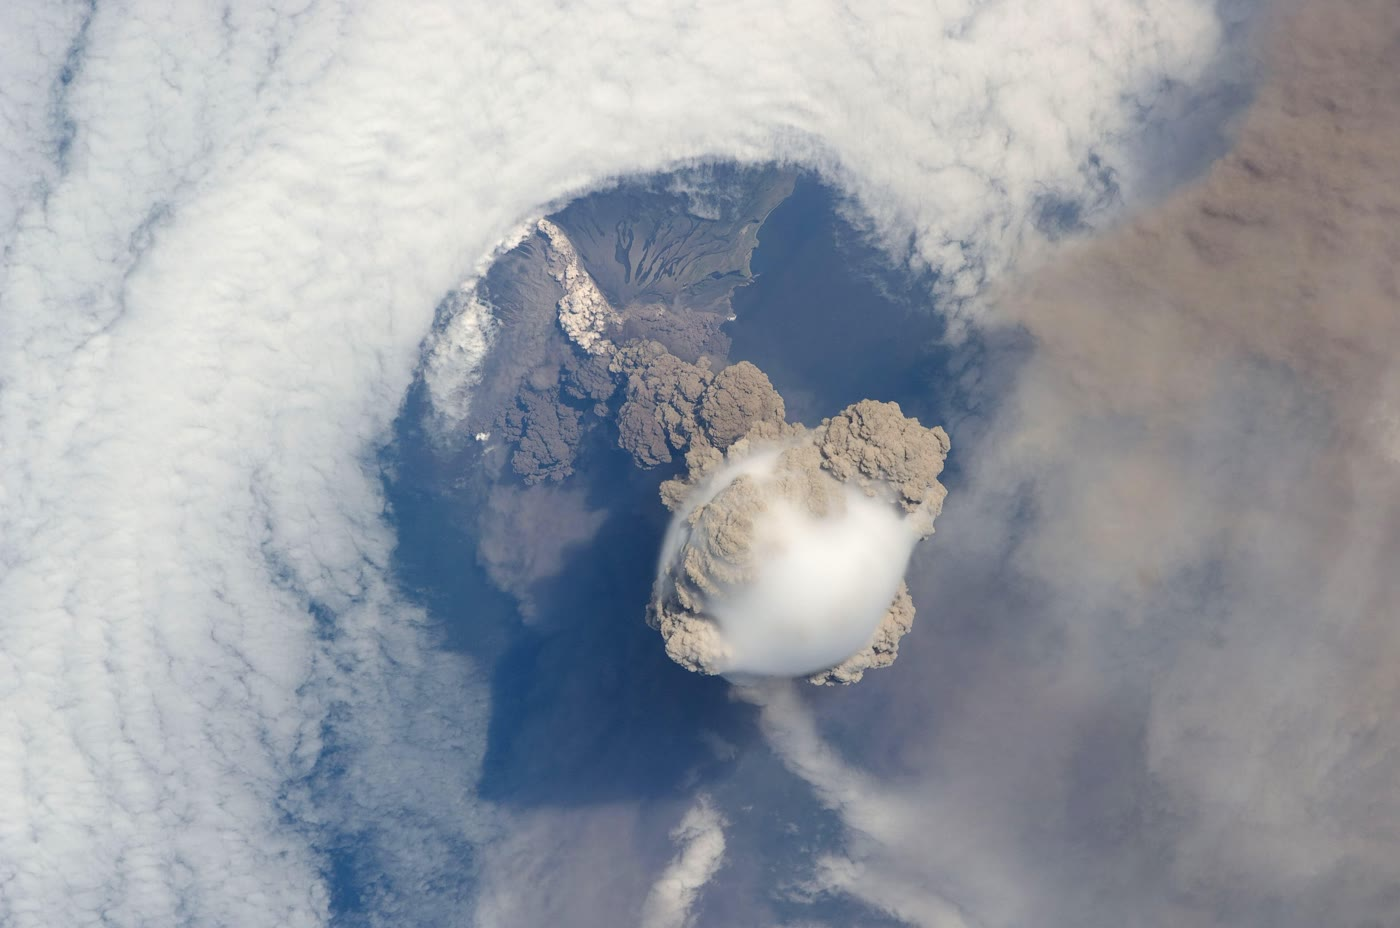
\includegraphics[width=0.66\linewidth]{images/book3/b1-sarychev-iss.jpg}
\par\smallskip{\small Sarychevpiek, een vulkaan van de Koerilese boog op het eiland Matua, in een vroeg stadium van de uitbarsting op 12 juni 2009, gezien vanuit het Internationaal Ruimtestation door een gat in de wolken. Grijze as, waarschijnlijk een pyroclastische stroom, loopt van de top naar beneden, en een gladde wolkenkap, een pileus, zit op de opstijgende zuil; as van de uitbarsting werd meer dan \qty{2400}{km} verder gedetecteerd. Foto: NASA, publiek domein (Wikimedia Commons).}
\label{fig:b1:active-margins:sarychev}
\end{omfigure}
% ledger: nasa:sarychev, commons:sarychev

De \omterm{def:b1:layered-earth:layers}{korst} onder bogen wordt verdikt, zowel door verkorting als door het magma dat van onderaf wordt toegevoegd; onder de bogen die op continenten zijn gebouwd, zoals de Andes, behoort zij tot de dikste van de aarde.

Achter sommige bogen wordt de bovenliggende plaat uit elkaar getrokken. Dan Karig verklaarde deze randbekkens van de westelijke Stille Oceaan in 1971 binnen de plaattektoniek: wanneer de plaatzijde steil zinkt en terugrolt, migreren de trog en de boog naar de zinkende plaat toe, en wordt de plaat erachter uitgerekt tot zij splijt, soms met een uitgestorven overblijfsel van de boog aan de andere kant. In het plaatmodel dat hierboven is gebruikt, loopt de achterboogspreiding op ongeveer \qty{32}{mm.yr^{-1}} in de Marianentrog nabij \ang{18}\,N, en met meer dan \qty{110}{mm.yr^{-1}} in het noorden van het Lau-bekken, achter Tonga. Waar de plaatzijde daarentegen ondiep ligt, sleept zij de bovenliggende plaat mee, waarvan de \omterm{def:b1:layered-earth:layers}{korst} achter de boog wordt verkort en verdikt, zoals achter de Andes.
% ledger: karig:marginal-basins, data:pb2002 (ridge_budget.py: Mariana 32.4, Lau 117.5 mm/yr)

\begin{inthefield}[Waarschuwing voor een tsunami]
Een centrum voor tsunamiwaarschuwing heeft enkele minuten. In 2011 kwam de eerste waarschuwing voor de kust van het noordoosten van Japan ongeveer drie minuten na de aardbeving, op basis van een magnitude die op de korteperiode seismische golven rustte; voor aardbevingen van magnitude 8 of meer wordt zo'n magnitude onderschat, en daarmee ook de hoogte van de tsunami. De momentmagnitude, die niet verzadigt, had ongeveer vijftien minuten nodig: de breedbandseismometers van Japan waren buiten hun bereik gedreven. Sinds 2013, toen de grootte van zo'n zware aardbeving onzeker is, gaat de eerste waarschuwing uit van de grootste aardbeving die daar mogelijk is, en beschrijft zij de tsunami met woorden, zoals ``enorm'', in plaats van met een getal; en de voorspellingen steunen op metingen op zee zelf, van boeien die via satelliet zijn gepositioneerd en drukmeters op de zeebodem, die de golf zien voordat zij de kust bereikt.
% ledger: jma:warning

\smallskip
\begin{center}
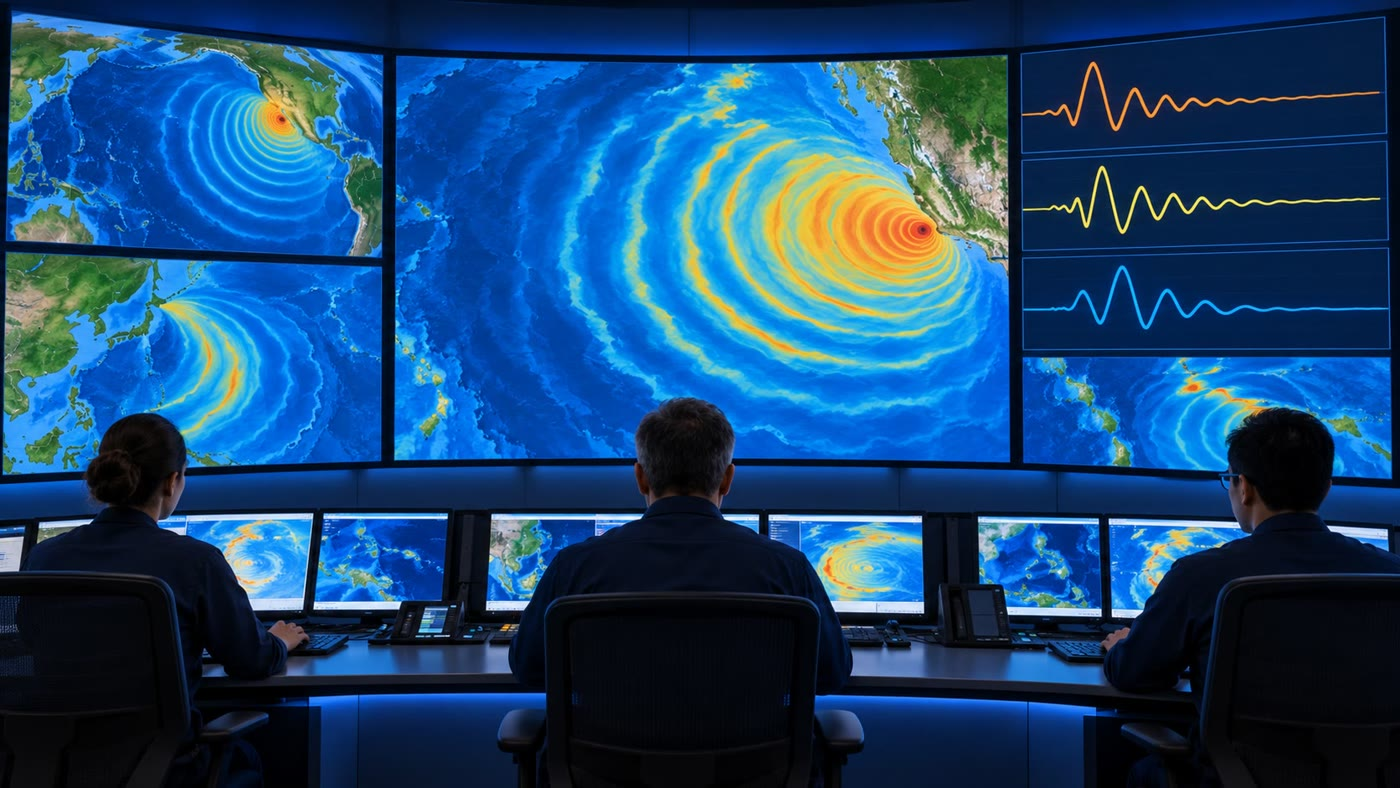
\includegraphics[width=0.7\linewidth]{images/book3/ai/b1-tsunami-centre.jpg}

{\scriptsize Dienstdoende functionarissen in een centrum voor tsunamiwaarschuwing, voor schermen met berekende golffronten en registraties van de zeespiegel (door AI gegenereerde illustratie).}
\end{center}
\end{inthefield}

\section{Oefeningen}

\begin{exercise}[$\star$]\label{exo:b1:active-margins:1}
Een trog ligt \qty{3}{km} onder de zeebodem eromheen. (a) Als zij niet gecompenseerd was, met hoeveel zou de zwaartekracht daar dalen door het ontbrekende gesteente, van dichtheid \qty{2700}{kg.m^{-3}}, dat door zeewater van dichtheid \qty{1000}{kg.m^{-3}} wordt vervangen? Gebruik de Bouguer-plaat, met $G = \qty{6.674e-11}{m^3.kg^{-1}.s^{-2}}$. (b) Vergelijk met de waargenomen anomalie boven de Koerilentrog, ongeveer \qty{-260}{\milli\gal}, waar de trog \qty{3.5}{km} onder de bodem eromheen ligt: herhaal de berekening voor die diepte. (c) Waarom geeft het water in een trog die slechts tientallen kilometers breed is minder dan de formule van de plaatzijde, en waar moet het overige tekort liggen?
\end{exercise}

\begin{exercise}[$\star$]\label{exo:b1:active-margins:2}
De Pacifische plaat komt de Koerilentrog binnen met \qty{82}{mm.yr^{-1}}. (a) Welke lengte van plaat zakt in 10 miljoen jaar weg? (b) Als de plaatzijde langs een rechte weg onder \ang{45} zonk, hoe diep zou haar voorrand dan zijn? (c) Hoe lang duurt het om \qty{600}{km} te bereiken?
\end{exercise}

\begin{exercise}[$\star$]\label{exo:b1:active-margins:3}
Vulkanen staan boven de plaats waar een rechte plaatzijde \qty{110}{km} diep is. Bereken de \omterm{def:b1:active-margins:volcanic-arc}{boog--trog-afstand} voor een plaatzijde die onder \ang{30}, \ang{45} en \ang{60} helt. Welke boog ligt het verst van zijn trog?
\end{exercise}

\begin{exercise}[$\star$]\label{exo:b1:active-margins:4}
In het digitale plaatmodel van het hoofdstuk gaan elk jaar ongeveer \qty{2.7}{km^2} oceaanbodem langs de subductiegrenzen naar beneden, langs ongeveer \qty{51000}{km}, en worden ongeveer \qty{3.0}{km^2} gemaakt langs ongeveer \qty{67000}{km} spreidingsruggen. (a) Bereken de gemiddelde convergentiesnelheid en de gemiddelde volledige spreidingssnelheid, in \unit{mm.yr^{-1}}. (b) Over al zijn grenzen vernietigt het model bijna evenveel oppervlak als het maakt. Waar gaat de rest van de nieuwe bodem heen?
% ledger: data:pb2002 (ridge_budget.py: 2.739 km2 over 51471 km; 3.009 km2 over 67340 km; all 3.511 vs 3.519)
\end{exercise}

\begin{exercise}[$\star\star$]\label{exo:b1:active-margins:5}
Vier aardbevingen van een doorsnede liggen op $(x, z) = (200, 150)$, $(300, 250)$, $(400, 330)$ en $(500, 430)$, in kilometer. (a) Pas de plaatzijdelijn met kleinste kwadraten en geef haar helling. (b) Waar bereikt de lijn het oppervlak? (c) Vergelijk met de helling van de lijn door alleen de eerste en de laatste aardbeving.
\end{exercise}

\begin{exercise}[$\star\star$]\label{exo:b1:active-margins:6}
Een model van een plaatzijde helt \ang{25} vanaf de trog tot \qty{50}{km} diep, en daarna onder \ang{45}. Het vulkanische front staat boven de plaats waar de plaatzijde \qty{110}{km} diep is. (a) Bereken de \omterm{def:b1:active-margins:volcanic-arc}{boog--trog-afstand}. (b) Vergelijk met een plaatzijde die overal onder \ang{45} helt. (c) Het diepe segment, naar boven doorgetrokken, bereikt het oppervlak: waar? Vergelijk met de Koerilese lijn, die het \qty{53}{km} landwaarts van de trog bereikt. (d) Welke kloof zou een diep segment van \ang{60} geven?
\end{exercise}

\begin{exercise}[$\star\star$]\label{exo:b1:active-margins:7}
(a) Welke hoekstraal, en welke straal in kilometer ($R = \qty{6371}{km}$), zou een boog volgens de propositie over het gebogen bolvormige oppervlak moeten hebben boven een plaatzijde die onder \ang{45} zinkt? \ang{30}? \ang{70}? (b) Welke bogen zijn het sterkst gekromd? (c) De Koerilese plaatzijde helt \ang{44.9} en de Koerilentrog past op een cirkel van \ang{21.9}: bereken het relatieve verschil met de voorspelling.
\end{exercise}

\begin{exercise}[$\star\star$]\label{exo:b1:active-margins:8}
Neem een geleidbaarheid van \qty{2.5}{W.m^{-1}.K^{-1}} en een oppervlaktetemperatuur van \qty{10}{\celsius}. (a) Bereken de oppervlaktetemperatuurgradiënt onder een \omterm{def:b1:active-margins:active-margin}{voorboog} die \qty{35}{mW.m^{-2}} verliest, en onder een \omterm{def:b1:active-margins:active-margin}{achterboogbekken} dat \qty{80}{mW.m^{-2}} verliest. (b) Extrapoleer deze gradiënten lineair en schat de temperatuur op \qty{30}{km} in elk. (c) Achterboogmohos zijn gemeten op 800 tot \qty{900}{\celsius}. Waarom is de lineaire schatting te hoog?
% ledger: hyndman:backarc (back-arc 70-85, Moho 800-900); the forearc value is an exercise value
\end{exercise}

\begin{exercise}[$\star\star$]\label{exo:b1:active-margins:9}
In het plaatmodel van het hoofdstuk opent de Marianentrog nabij \ang{18}\,N met een volledige snelheid van ongeveer \qty{32}{mm.yr^{-1}}. (a) Druk deze snelheid uit in \unit{km.Myr^{-1}}, en geef de halve snelheid als de spreiding symmetrisch is. (b) Hoe lang zou de trog erover doen om met \qty{100}{km} te openen tegen dit tempo? (c) Geef twee redenen waarom de leeftijd van een \omterm{def:b1:active-margins:active-margin}{achterboogbekken} niet eenvoudig uit zijn breedte en zijn huidige snelheid kan worden afgelezen.
% ledger: data:pb2002 (ridge_budget.py: mariana_18n_mm_yr 32.4)
\end{exercise}

\begin{exercise}[$\star\star\star$]\label{exo:b1:active-margins:10}
Een plaatzijde van \qty{100}{km} dik zinkt met \qty{82}{mm.yr^{-1}} langs een traject dat onder \ang{45} helt. Neem $\kappa = \qty{e-6}{m^2.s^{-1}}$. (a) Hoe lang duurt het om \qty{600}{km} te bereiken? (b) Hoe ver diffundeert warmte er in die tijd in, volgens $\sqrt{\kappa t}$? (c) Hoe lang zou warmte erover doen om haar midden te bereiken? (d) Concludeer over de temperatuur van de plaatzijde op \qty{600}{km} en over haar aardbevingen.
\end{exercise}

\begin{exercise}[$\star\star\star$]\label{exo:b1:active-margins:11}
Een model van een \omterm{def:b1:active-margins:accretionary}{accretionair prisma} heeft een driehoekige doorsnede: zijn oppervlak helt onder $\alpha = \ang{4}$ naar de trog en zijn basis helt onder $\beta = \ang{6}$ eronder, beide komen samen aan zijn teen; hij behoudt deze hoeken terwijl hij groeit. (a) Toon aan dat zijn oppervlakte $A = \frac12 L^2(\tan\alpha + \tan\beta)$ is voor een breedte $L$, wanneer de hoeken klein genoeg zijn opdat de hoogte aan de achterkant $L(\tan\alpha + \tan\beta)$ is. (b) Sediment van \qty{1}{km} dik komt aan op een plaat die met \qty{40}{mm.yr^{-1}} convergeert, en al het sediment wordt geaccreteerd: bereken de breedte na 1, 4 en 10 miljoen jaar. Hoe groeit $L$ met de tijd? (c) Wat als de helft van het sediment met de plaatzijde naar beneden gaat?
\end{exercise}

\begin{exercise}[$\star\star\star$]\label{exo:b1:active-margins:12}
(a) Toon aan dat de kleinste-kwadratenlijn door het gemiddelde punt $(\bar x, \bar z)$ gaat. (b) Een catalogus geeft elke diepte \qty{10}{km} te diep. Hoe veranderen de helling en het snijpunt van de gepaste lijn? (c) De afstanden $x$ zijn alle gemeten vanaf een punt op de trog dat \qty{20}{km} te ver landwaarts is geplaatst, zodat elke $x$ \qty{20}{km} te klein is. Hoe veranderen de helling en het snijpunt? (d) Verandert een van beide fouten de helling?
\end{exercise}

\section{Probleem: een subductiezone lezen uit haar aardbevingen}

\begin{problem}[{Weekendprobleem --- de Koerilese plaatzijde uit acht aardbevingen, hoe snel zij zakt, wat haar zwaartekracht en warmtestroom zeggen, en waar haar vulkanen zouden moeten staan}]
\label{pb:b1:active-margins:1}
% values: calc/ch14.py; the eight events are real (USGS catalogue, rounded to the km)
% from figdata/out/bachelor-1-slab_seismicity-section.dat
% ledger: data:b3-usgs-kuril, data:pb2002, data:b2-seafloor-age, syracuse:arc-depth, frank:arcs,
% data:b3-grav-kuril, parsons:plate-model, hyndman:backarc; the forearc heat flow is an exercise value
Acht aardbevingen van de Koerilese plaatzijde, alle dieper dan \qty{70}{km}, zijn opgesomd naar hun afstand $x$ tot de trog langs de doorsnedelijn, richting de Okhotskzee, en hun diepte $z$, beide afgerond op de kilometer.

\begin{center}
\small
\begin{tabular}{lcccccccc}
\hline
gebeurtenis & 1 & 2 & 3 & 4 & 5 & 6 & 7 & 8\\
$x$ (\unit{km}) & 155 & 222 & 305 & 319 & 431 & 533 & 578 & 609\\
$z$ (\unit{km}) & 96 & 169 & 245 & 272 & 389 & 489 & 518 & 573\\
magnitude & 5.5 & 5.1 & 5.0 & 5.4 & 5.3 & 5.3 & 5.2 & 6.4\\
\hline
\end{tabular}
\end{center}

\medskip
\noindent\textbf{Deel I --- De plaatzijdelijn.}
\begin{enumerate}
  \item Zet de acht aardbevingen op dezelfde schaal op beide assen, met de diepte naar beneden.
  \item Bereken $\sum x_i$, $\sum z_i$, $\sum x_i^2$, $\sum x_i z_i$ en de gemiddelden $\bar x$ en $\bar z$.
  \item Bereken $S_{xx}$ en $S_{xz}$, en daarna de helling van de kleinste-kwadratenlijn tot op drie decimalen en haar snijpunt tot op één decimaal.
  \item Hoe groot is de helling van de plaatzijde?
  \item Waar bereikt de lijn het oppervlak? Wat zegt dit over de vorm van de plaatzijde nabij de trog?
  \item Bereken de afwijking $z_i - (a + s x_i)$ van elke aardbeving. Welke liggen het verst van de lijn, en hoe ver?
\end{enumerate}

\medskip
\noindent\textbf{Deel II --- Hoe snel de plaatzijde zakt.} Aan het begin van de doorsnede geeft het PB2002-model een convergentie van \qty{87.4}{mm.yr^{-1}}: ten opzichte van de Okhotskplaat beweegt de Pacifische plaat naar \omterm{def:b1:spherical-astronomy:horizontal}{azimut} \ang{300}. De doorsnedelijn, loodrecht op de trog, loopt naar \omterm{def:b1:spherical-astronomy:horizontal}{azimut} \ang{320.9}.
\begin{enumerate}[resume]
  \item Bereken de hoek tussen de convergentie en de doorsnedelijn, en daarna de componenten van de convergentie loodrecht op en evenwijdig aan de trog.
  \item Welke lengte van plaat zakt in 10 miljoen jaar de trog in?
  \item Gebruik de helling van vraag 4 (afgerond op \ang{45}): hoe lang doet de plaatzijde erover om een punt van haar bovenkant van de trog naar de diepste aardbeving van de band, op \qty{632}{km}, te brengen? Verwaarloos de flauwere helling nabij de trog.
  \item De plaat is bij de trog ongeveer \qty{122}{Myr} oud. Hoe oud is de zeebodem die nu \qty{632}{km} diep ligt?
  \item Hoe ver is warmte bij $\sqrt{\kappa t}$, met $\kappa = \qty{e-6}{m^2.s^{-1}}$, tijdens die afdaling in de plaatzijde gediffundeerd? Vergelijk met haar dikte, ongeveer \qty{100}{km}.
\end{enumerate}

\medskip
\noindent\textbf{Deel III --- Zwaartekracht en warmtestroom.} Neem een geleidbaarheid van \qty{2.5}{W.m^{-1}.K^{-1}}.
\begin{enumerate}[resume]
  \item De oude oceaanbodem voor de trog verliest ongeveer \qty{43}{mW.m^{-2}}, het \omterm{def:b1:active-margins:active-margin}{achterboogbekken} ongeveer \qty{80}{mW.m^{-2}}; neem \qty{35}{mW.m^{-2}} voor de \omterm{def:b1:active-margins:active-margin}{voorboog}. Bereken de temperatuurgradiënt nabij het oppervlak van elk.
  \item Verklaar waarom de \omterm{def:b1:active-margins:active-margin}{voorboog} minder warmte verliest dan de oude oceaanbodem ervoor.
  \item De \omterm{def:b1:isostasy-gravity:anomalies}{vrije-luchtanomalie} boven de Koerilentrog is ongeveer \qty{-260}{\milli\gal}. Welke dikte gesteente van \qty{1700}{kg.m^{-3}} dichter dan water zou een Bouguer-plaat nodig hebben om dit tekort te geven? Vergelijk met de diepte van de trog onder de bodem eromheen, ongeveer \qty{3.5}{km}.
  \item Stel nu dat de hele plaat \qty{3.5}{km} naar beneden wordt gedrukt: water neemt de plaats in van gesteente aan haar bovenkant, en haar \omterm{def:b1:layered-earth:layers}{korst} die van de \omterm{def:b1:layered-earth:layers}{mantel} aan haar basis, zodat in het geheel \omterm{def:b1:layered-earth:layers}{mantel} van dichtheid \qty{3300}{kg.m^{-3}} door water wordt vervangen. Bereken de anomalie van de Bouguer-plaat. Waarom geeft de echte trog, die slechts tientallen kilometers breed is, minder?
  \item De trog en de buitenrug zijn niet in isostatisch evenwicht. Wat houdt hen daaruit?
\end{enumerate}

\medskip
\noindent\textbf{Deel IV --- Waar de vulkanen zouden moeten staan.} Gebruik de lijn van vraag 3, met haar afgeronde helling en snijpunt.
\begin{enumerate}[resume]
  \item De eerste vulkaan van de band ligt \qty{164}{km} van de trog. Hoe diep is de plaatzijde eronder?
  \item Ligt deze diepte binnen het bereik dat onder bogen is gevonden, 72 tot \qty{173}{km}? Hoe ver ligt zij van het gemiddelde, \qty{105}{km}?
  \item Op welke afstand van de trog is de plaatzijde \qty{100}{km} diep?
  \item Welke hoekstraal, volgens de propositie over het gebogen bolvormige oppervlak, zou de Koerilese boog moeten hebben, en welke straal in kilometers?
  \item De Koerilentrog past op een \omterm{def:b1:spherical-astronomy:spherical-triangle}{kleine cirkel} van \ang{21.9}. Vergelijk.
  \item Vulkanen van bogen staan gemiddeld waar de plaatzijde ongeveer \qty{105}{km} diep is. Op welke afstand van de trog bereikt de plaatzijde-lijn die diepte?
  \item Vergelijk deze afstand met de waargenomen \qty{164}{km}: met hoeveel kilometer en met welke fractie verschilt zij?
  \item Tot op de kilometer nauwkeurig, welke \omterm{def:b1:active-margins:volcanic-arc}{boog--trog-afstand} voorspelt de lijn van de Koerilese plaatzijde voor vulkanen die op \qty{105}{km} boven de plaatzijde staan?
\end{enumerate}
\end{problem}
